\documentclass[12pt]{article}
\usepackage{times} 			% use Times New Roman font

\usepackage[margin=1in]{geometry}   % sets 1 inch margins on all sides
\usepackage{hyperref}               % for URL formatting
\usepackage[pdftex]{graphicx}       % So includegraphics will work
\setlength{\parskip}{1em}           % skip 1em between paragraphs
\usepackage{indentfirst}            % indent the first line of each paragraph
\usepackage{datetime}
\usepackage[small, bf]{caption}
\usepackage{listings}               % for code listings
\usepackage{xcolor}                 % for styling code
\usepackage{multirow}
\usepackage{float}
\definecolor{backcolour}{RGB}{246, 246, 246}   % 0xF6, 0xF6, 0xF6
\definecolor{codegreen}{RGB}{16, 124, 2}       % 0x10, 0x7C, 0x02
\definecolor{codepurple}{RGB}{170, 0, 217}     % 0xAA, 0x00, 0xD9
\definecolor{codered}{RGB}{154, 0, 18}         % 0x9A, 0x00, 0x12

%Code listing style named "gcolabstyle" - matches Google Colab
\lstdefinestyle{gcolabstyle}{
  basicstyle=\ttfamily\small,
  backgroundcolor=\color{backcolour},   
  commentstyle=\itshape\color{codegreen},
  keywordstyle=\color{codepurple},
  stringstyle=\color{codered},
  numberstyle=\ttfamily\footnotesize\color{darkgray}, 
  breakatwhitespace=false,         
  breaklines=true,                 
  captionpos=b,                    
  keepspaces=true,                 
  numbers=left,                    
  numbersep=5pt,                  
  showspaces=false,                
  showstringspaces=false,
  showtabs=false,                  
  tabsize=2
}

\lstset{style=gcolabstyle}      %set gcolabstyle code listing

% to make long URIs break nicely
\makeatletter
\g@addto@macro{\UrlBreaks}{\UrlOrds}
\makeatother

% for fancy page headings
\usepackage{fancyhdr}
\setlength{\headheight}{13.6pt} % to remove fancyhdr warning
\pagestyle{fancy}
\fancyhf{}
\rhead{\small \thepage}
\lhead{\small HW5, Adeniran}  % EDIT THIS, REPLACE # with HW number
\chead{\small CS 532, Spring 2021} 

%-------------------------------------------------------------------------
\begin{document}

\begin{centering}
{\large\textbf{HW5 - Graph Partitioning}}\\ % EDIT THIS
                                % REPLACE # with HW num and ADD title
Adeniran Adeniyi\\                     % EDIT THIS
Sunday, March 28, 2021 by 11:59pm\\                      % EDIT THIS
\end{centering}

%-------------------------------------------------------------------------

% The * after \section just says to not number the sections
%----------------------------Q1111111111111111111111111111111111

\section*{Q1}
Draw the original Karate club graph (before the split) and color the nodes according to the factions they belong to (John A or Mr. Hi).
\subsection*{\color{blue}{Answer}}
\lstinputlisting[language=Python,caption=graphing.py, label=Q1:import,firstnumber=1,firstline=1,lastline=157]{graphing.py}

\begin{figure}[H]
\centering
% trim and clip are used to crop the image, trim=left bottom right top
% width sets max width, height will be scaled appropriately
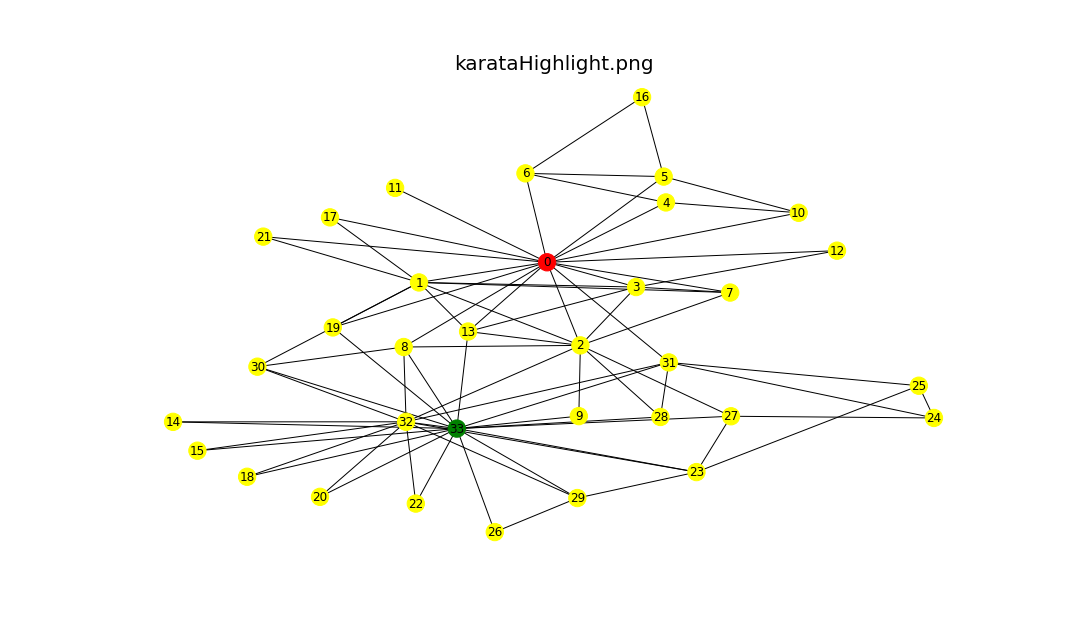
\includegraphics[trim=0 0 0 0, clip, width=\textwidth] {karataHighlight.png}
\caption{Dataset with two main  group highlighted Red(John A), Green (My Hi), and Yellow for all others for visibility }
\label{fig:q1v}
\end{figure}
\begin{figure}[H]
\centering
% trim and clip are used to crop the image, trim=left bottom right top
% width sets max width, height will be scaled appropriately
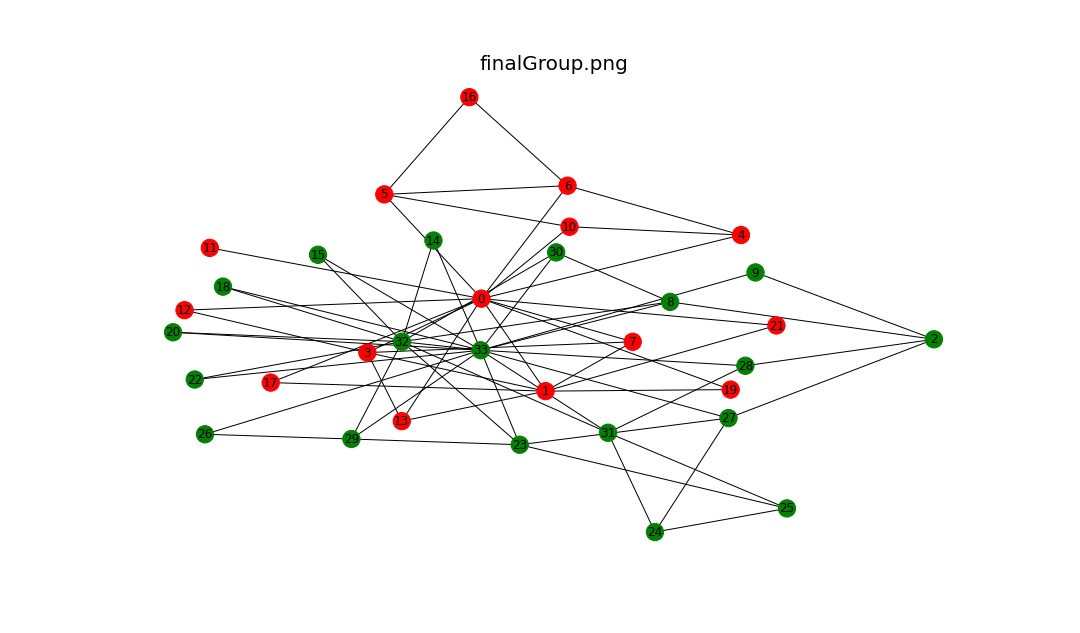
\includegraphics[trim=0 0 0 0, clip, width=\textwidth] {finalGroup.png}
\caption{Appropriately distritbuted node colors, edges still as it is}
\label{fig:q1d}
\end{figure}


\emph{}
\subsection*{Discussion}
\emph{I used networkx library, where the Zachary Karate club dataset is on.}
\lstinputlisting[language=Python,caption=Getting data from networkx snapcshto of graphing.py, label=Q1a:import,firstnumber=122,firstline=122,lastline=122]{graphing.py}
\emph{
For this graph, I highlighed the two major parts of the Zachary karate club Main Leader, John A which represents the Red color and node number 0, while Mr Hi represent the color green and node number 33. They reset are will be given a color yellow for more visibility.\\
Major parts that ensured the result are reflect in the code snapshot of graphing.py:}
    \begin{itemize}
        \item The driver for the question \lstinputlisting[language=Python,caption=graphing.py, label=Q1b:import,firstnumber=124,firstline=124,lastline=135]{graphing.py}
        \item colorCode function builds the list of the color for each nodes 
        \lstinputlisting[language=Python,caption=Building list for the color node in the graph (snapshot in graphing.py), label=Q1c:import,firstnumber=25,firstline=25,lastline=39]{graphing.py}
        \item A graphing function that handles all my graphing needs. For this part, I used the first conditional statement in line 69 -70
         \lstinputlisting[language=Python,caption= Making the plot for all the graphs (snapshot in graphing.py), label=Q1d:import,firstnumber=64,firstline=64,lastline=79]{graphing.py}
    \end{itemize}

\section*{Q2}
Run multiple iterations of the Girvan-Newman graph partioning algorithm (see Week-07 Social Networks, slides 90-99) on the Karate Club graph until the graph splits into two connected components. Keep the node colors the same as they were set in Q1. How many iterations did it take? \\ 
Your report should include images of all of the iterations. It will be easier to see the splits if you use a force-directed layout (such as Kamada-Kawai) rather than a circular layout. \\ \\ \\
\subsection*{\color{blue}{Answer}}
\lstinputlisting[language=Python,caption=Girvan-newman algorithm (snapshot of graphing.py), label=Q1e:import,firstnumber=96,firstline=96,lastline=119]{graphing.py}

\begin{figure}[H]
\centering
% trim and clip are used to crop the image, trim=left bottom right top
% width sets max width, height will be scaled appropriately
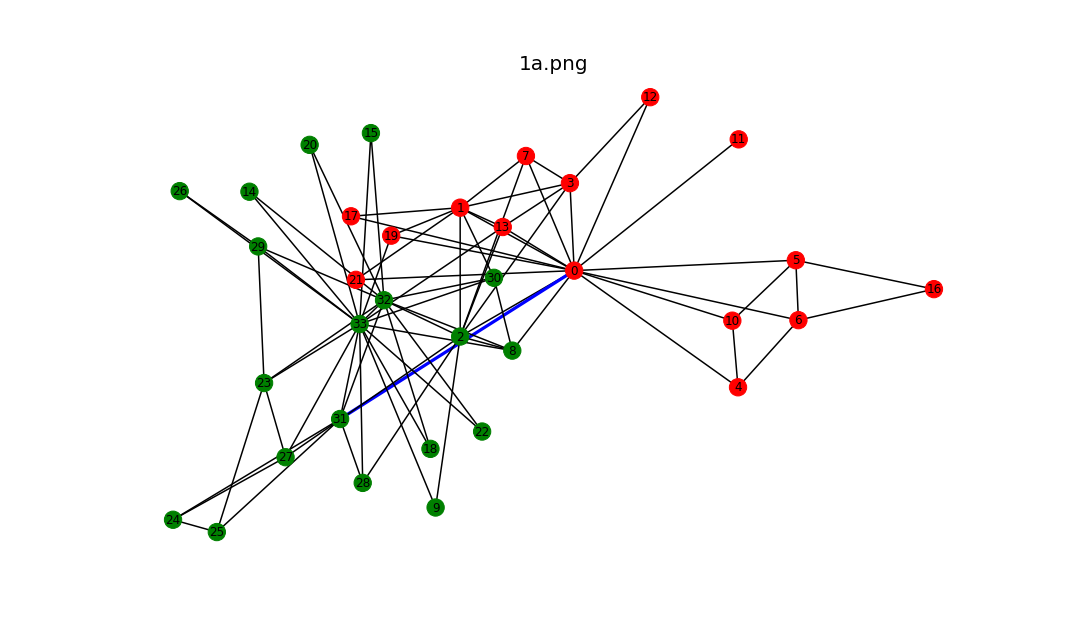
\includegraphics[trim=0 0 0 0, clip, width=\textwidth] {1a.png}
\caption{Iteration 1 Highlighted nodeedge to remove in blue }
\label{fig:q11a}
\end{figure}

\begin{figure}[H]
\centering
% trim and clip are used to crop the image, trim=left bottom right top
% width sets max width, height will be scaled appropriately
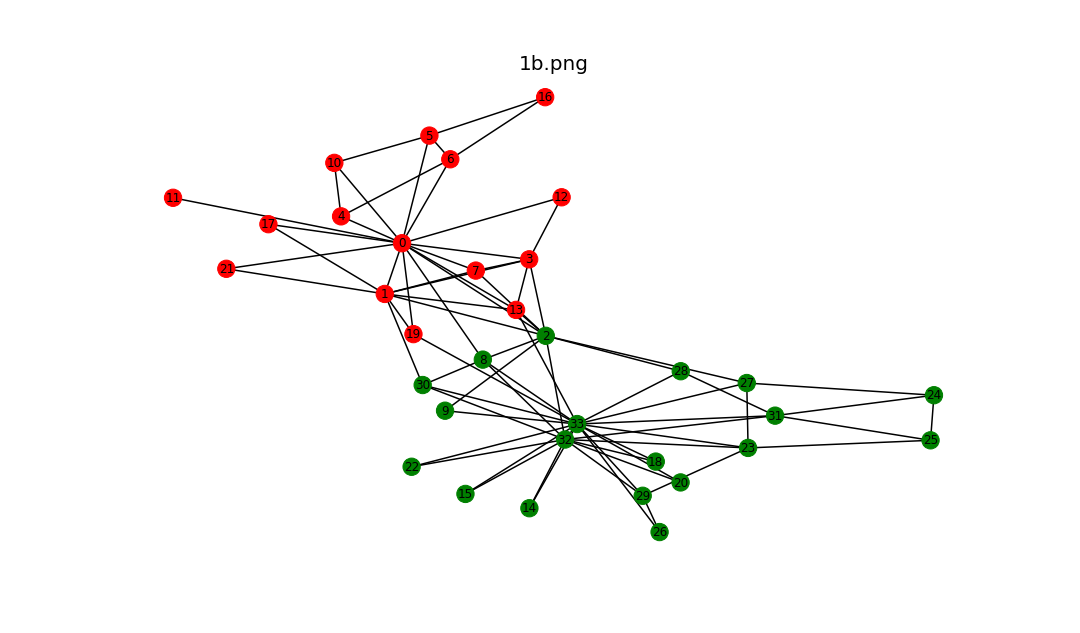
\includegraphics[trim=0 0 0 0, clip, width=\textwidth] {1b.png}
\caption{Iteration 1 confirm nodeedge has been removed }
\label{fig:q11b}
\end{figure}

\begin{figure}[H]
\centering
% trim and clip are used to crop the image, trim=left bottom right top
% width sets max width, height will be scaled appropriately
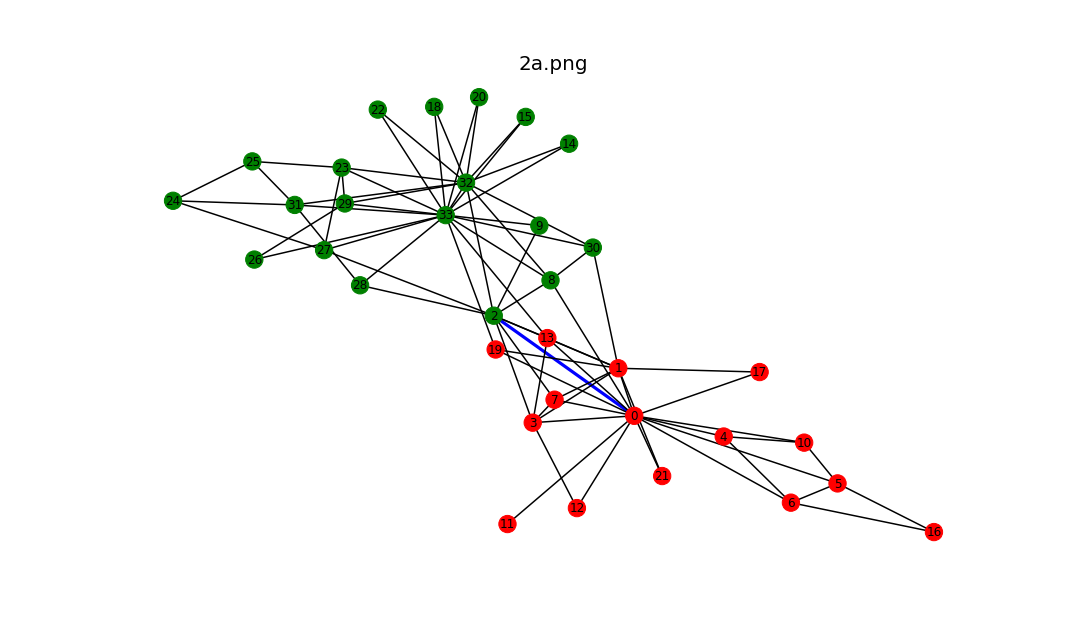
\includegraphics[trim=0 0 0 0, clip, width=\textwidth]{ 2a.png}
\caption{Iteration 2 Highlighted nodeedge to remove in blue }
\label{fig:q12a}
\end{figure}
\begin{figure}[H]
\centering
% trim and clip are used to crop the image, trim=left bottom right top
% width sets max width, height will be scaled appropriately
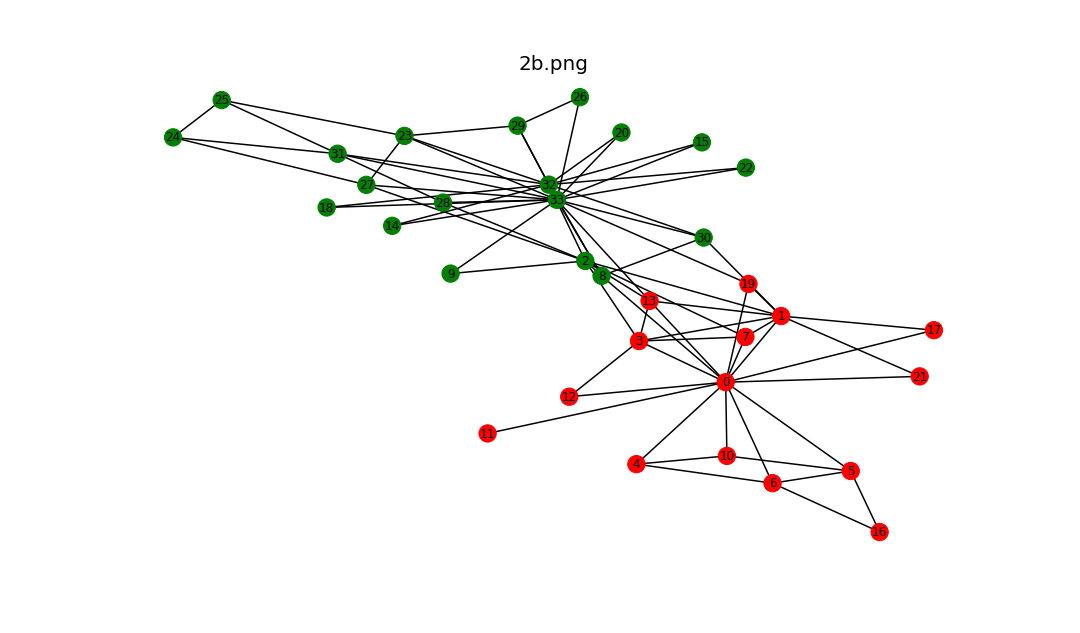
\includegraphics[trim=0 0 0 0, clip, width=\textwidth] {2b.png}
\caption{Iteration 2 confirm nodeedge has been removed }
\label{fig:q12b}
\end{figure}

\begin{figure}[H]
\centering
% trim and clip are used to crop the image, trim=left bottom right top
% width sets max width, height will be scaled appropriately
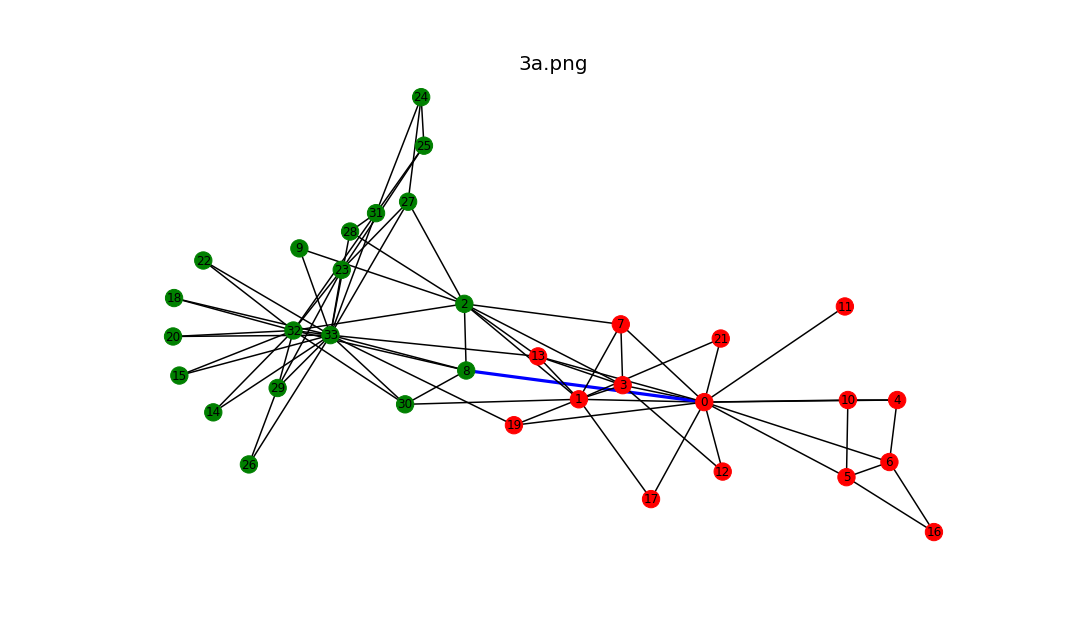
\includegraphics[trim=0 0 0 0, clip, width=\textwidth] {3a.png}
\caption{Iteration 3 Highlighted nodeedge to remove in blue }
\label{fig:q13a}
\end{figure}
\begin{figure}[H]
\centering
% trim and clip are used to crop the image, trim=left bottom right top
% width sets max width, height will be scaled appropriately
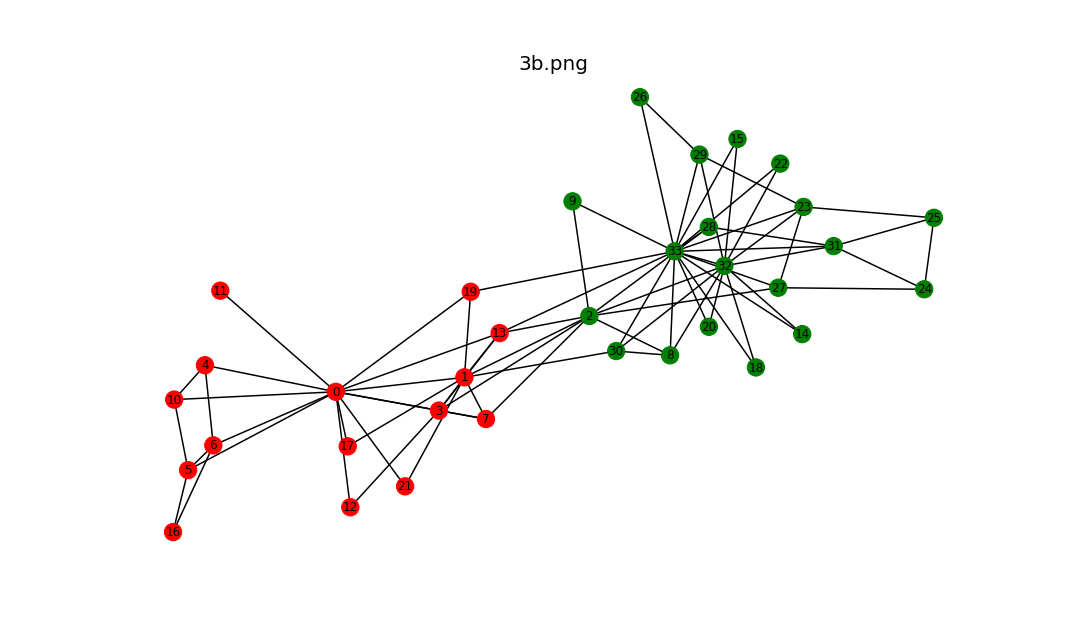
\includegraphics[trim=0 0 0 0, clip, width=\textwidth] {3b.png}
\caption{Iteration 3 confirm nodeedge has been removed }
\label{fig:q13b}
\end{figure}

\begin{figure}[H]
\centering
% trim and clip are used to crop the image, trim=left bottom right top
% width sets max width, height will be scaled appropriately
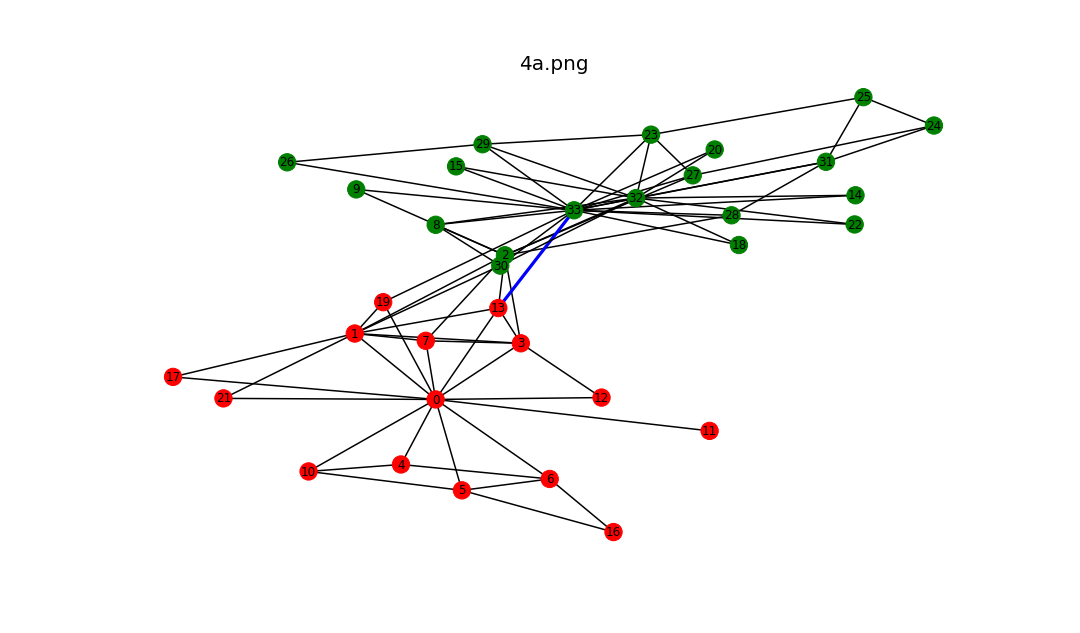
\includegraphics[trim=0 0 0 0, clip, width=\textwidth] {4a.png}
\caption{Iteration 4 Highlighted nodeedge to remove in blue }
\label{fig:q14a}
\end{figure}
\begin{figure}[H]
\centering
% trim and clip are used to crop the image, trim=left bottom right top
% width sets max width, height will be scaled appropriately
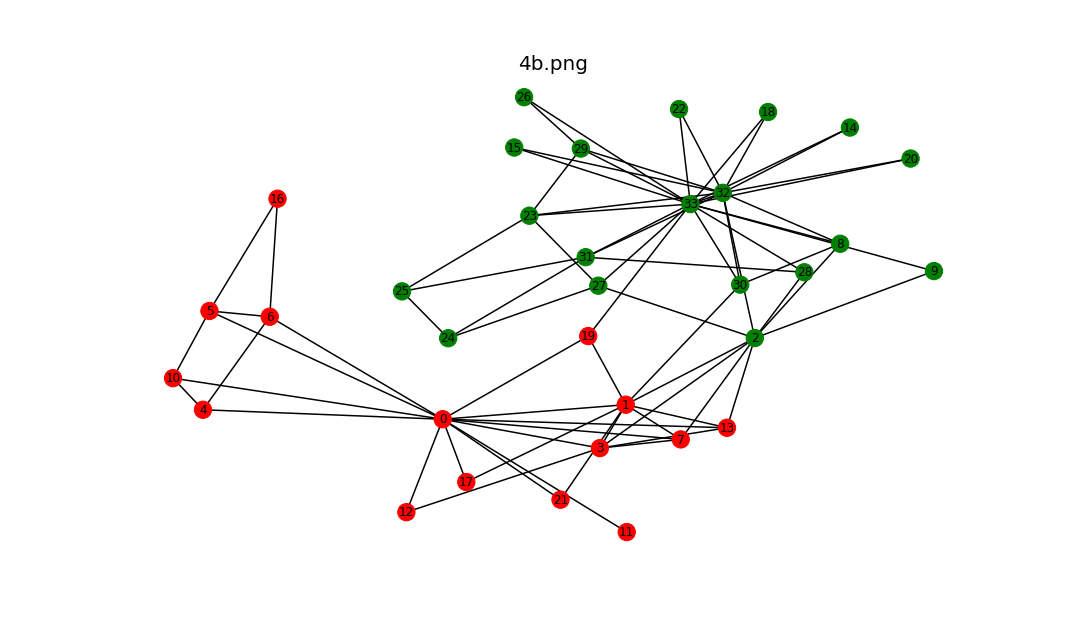
\includegraphics[trim=0 0 0 0, clip, width=\textwidth] {4b.png}
\caption{Iteration 4 confirm nodeedge has been removed }
\label{fig:q14b}
\end{figure}

\begin{figure}[H]
\centering
% trim and clip are used to crop the image, trim=left bottom right top
% width sets max width, height will be scaled appropriately
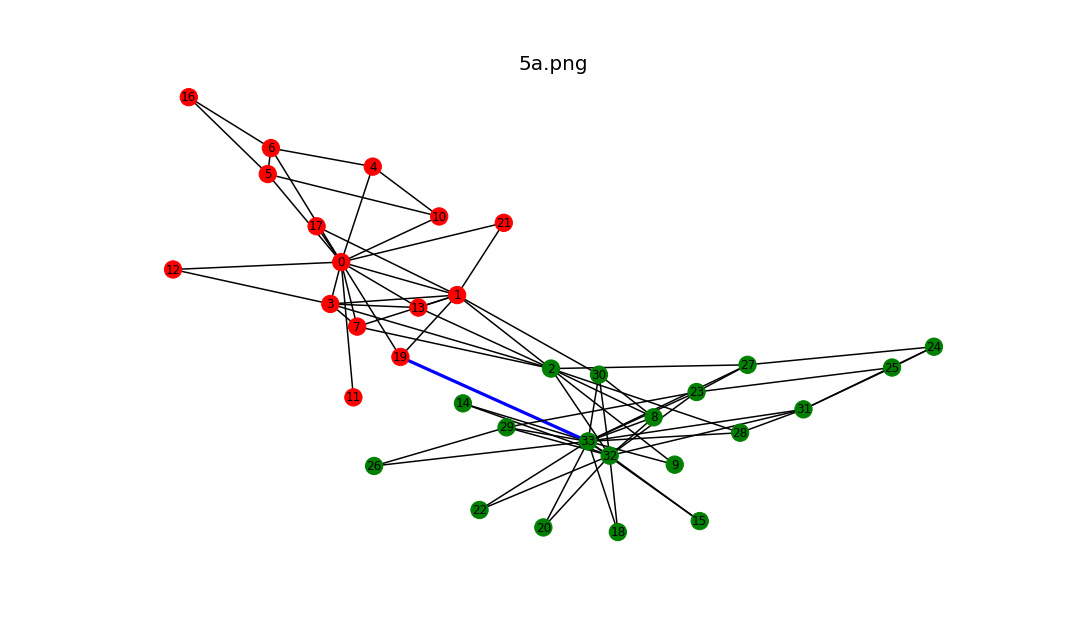
\includegraphics[trim=0 0 0 0, clip, width=\textwidth] {5a.png}
\caption{Iteration 5 Highlighted nodeedge to remove in blue }
\label{fig:q15a}
\end{figure}
\begin{figure}[H]
\centering
% trim and clip are used to crop the image, trim=left bottom right top
% width sets max width, height will be scaled appropriately
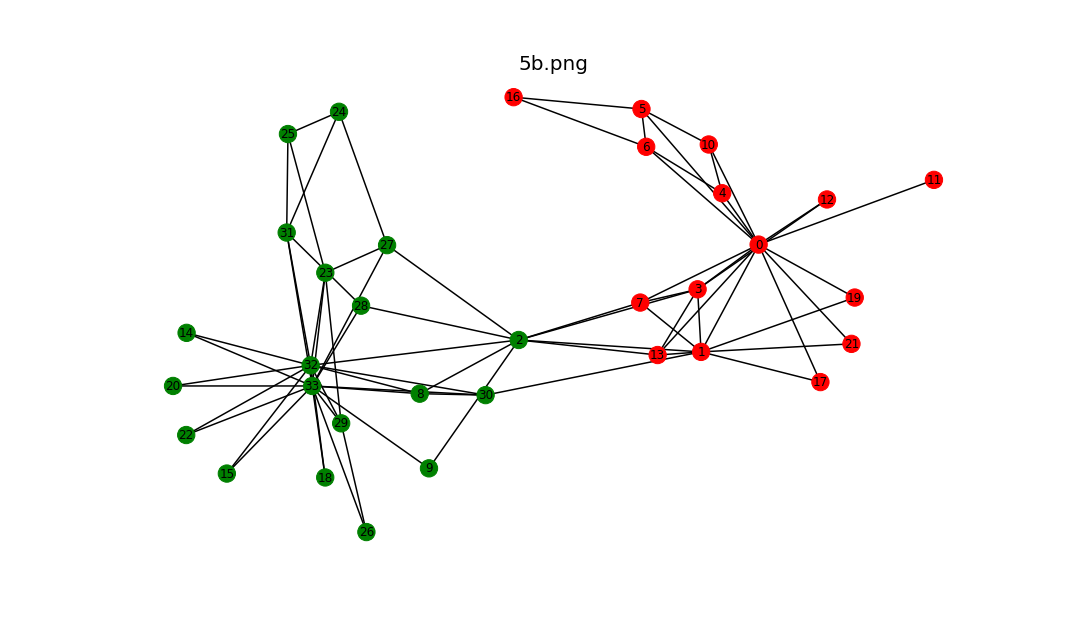
\includegraphics[trim=0 0 0 0, clip, width=\textwidth] {5b.png}
\caption{Iteration 5 confirm nodeedge has been removed }
\label{fig:q15b}
\end{figure}


\begin{figure}[H]
\centering
% trim and clip are used to crop the image, trim=left bottom right top
% width sets max width, height will be scaled appropriately
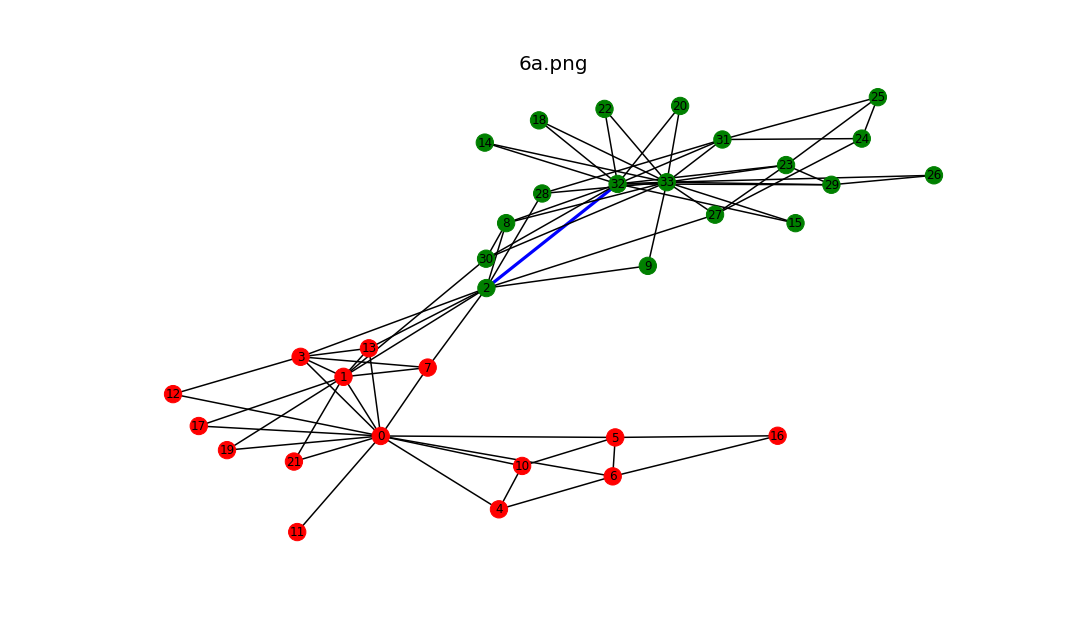
\includegraphics[trim=0 0 0 0, clip, width=\textwidth] {6a.png}
\caption{Iteration 6 Highlighted nodeedge to remove in blue }
\label{fig:q16a}
\end{figure}
\begin{figure}[H]
\centering
% trim and clip are used to crop the image, trim=left bottom right top
% width sets max width, height will be scaled appropriately
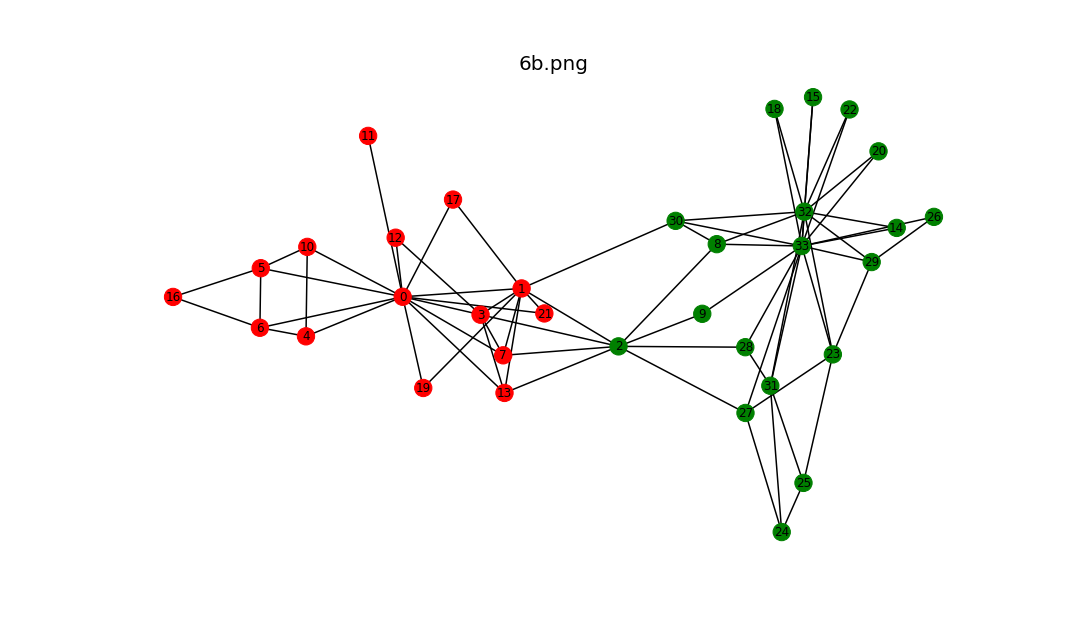
\includegraphics[trim=0 0 0 0, clip, width=\textwidth] {6b.png}
\caption{Iteration 6 confirm nodeedge has been removed }
\label{fig:q16b}
\end{figure}

\begin{figure}[H]
\centering
% trim and clip are used to crop the image, trim=left bottom right top
% width sets max width, height will be scaled appropriately
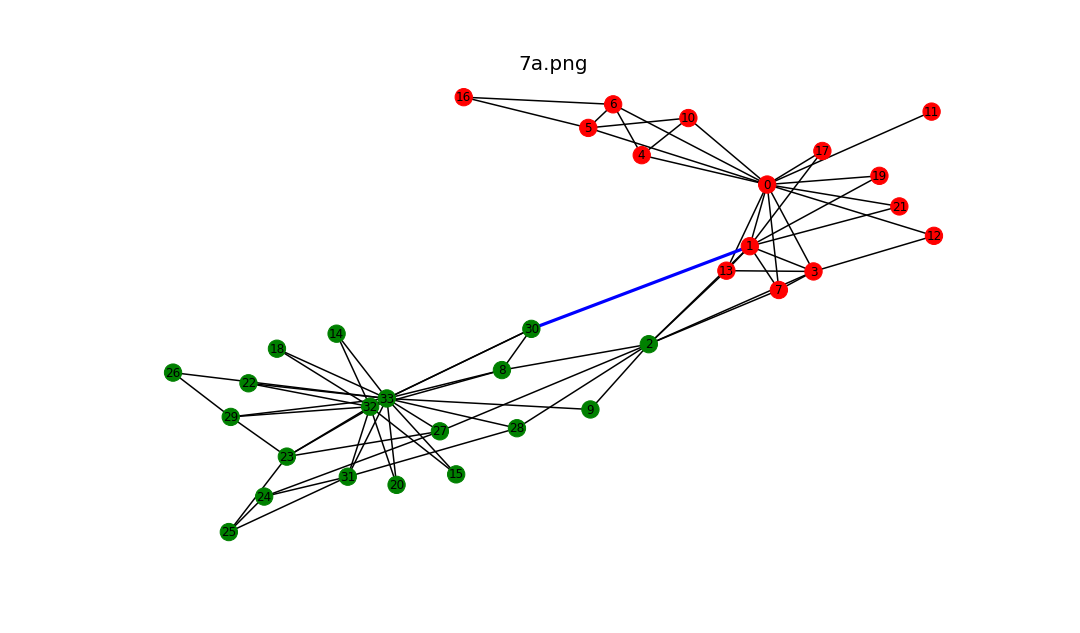
\includegraphics[trim=0 0 0 0, clip, width=\textwidth] {7a.png}
\caption{Iteration 7 Highlighted nodeedge to remove in blue }
\label{fig:q17a}
\end{figure}
\begin{figure}[H]
\centering
% trim and clip are used to crop the image, trim=left bottom right top
% width sets max width, height will be scaled appropriately
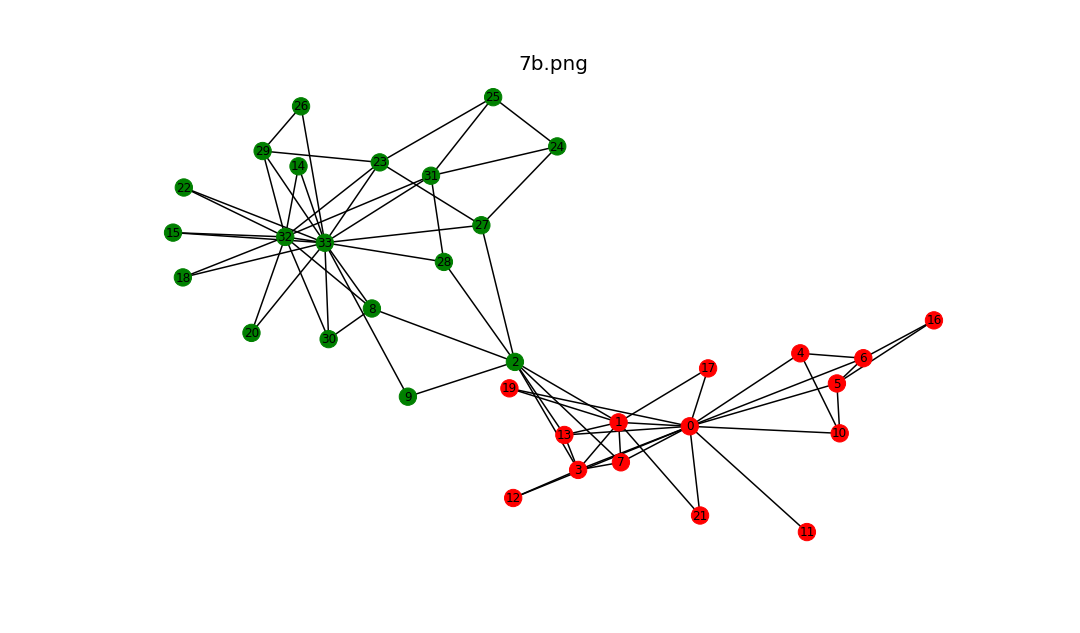
\includegraphics[trim=0 0 0 0, clip, width=\textwidth] {7b.png}
\caption{Iteration 7 confirm nodeedge has been removed }
\label{fig:q17b}
\end{figure}


\begin{figure}[H]
\centering
% trim and clip are used to crop the image, trim=left bottom right top
% width sets max width, height will be scaled appropriately
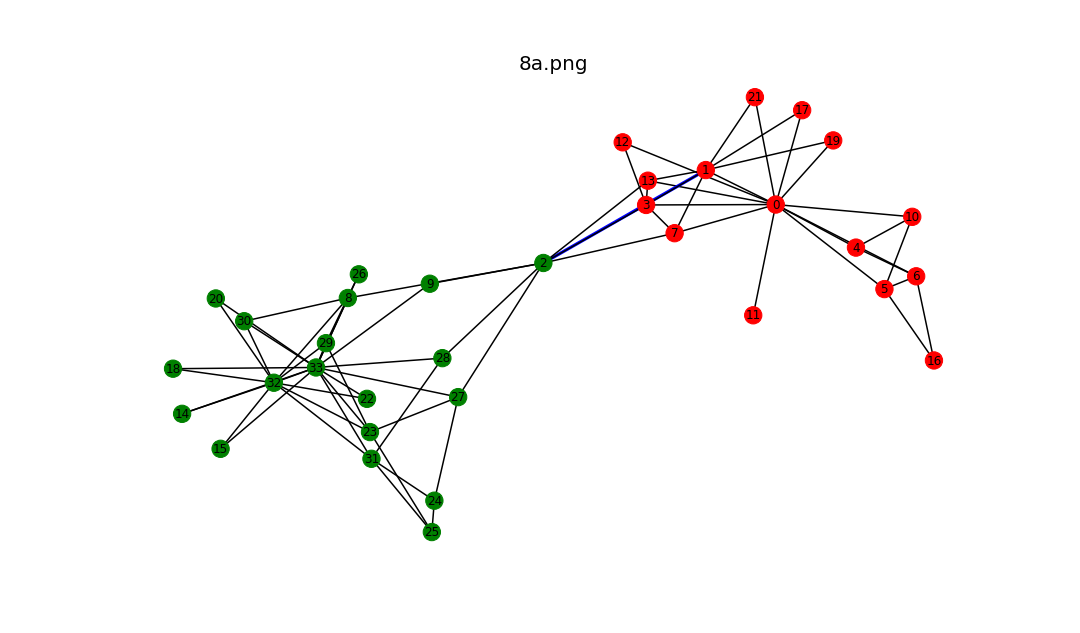
\includegraphics[trim=0 0 0 0, clip, width=\textwidth] {8a.png}
\caption{Iteration 8 Highlighted nodeedge to remove in blue }
\label{fig:q18a}
\end{figure}
\begin{figure}[H]
\centering
% trim and clip are used to crop the image, trim=left bottom right top
% width sets max width, height will be scaled appropriately
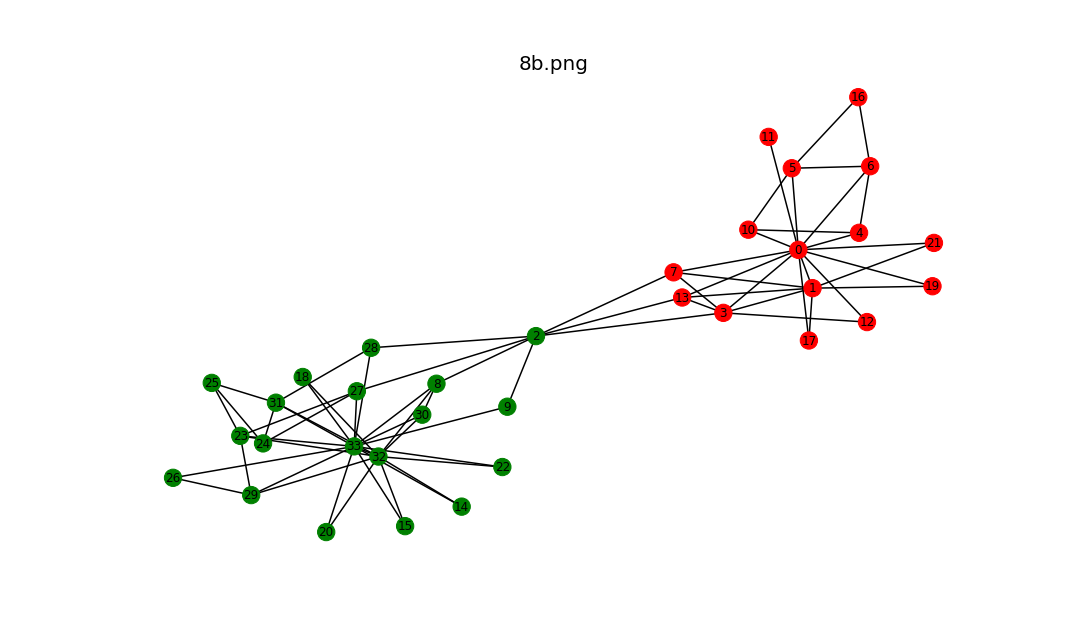
\includegraphics[trim=0 0 0 0, clip, width=\textwidth] {8b.png}
\caption{Iteration 8 confirm nodeedge has been removed }
\label{fig:q18b}
\end{figure}


\begin{figure}[H]
\centering
% trim and clip are used to crop the image, trim=left bottom right top
% width sets max width, height will be scaled appropriately
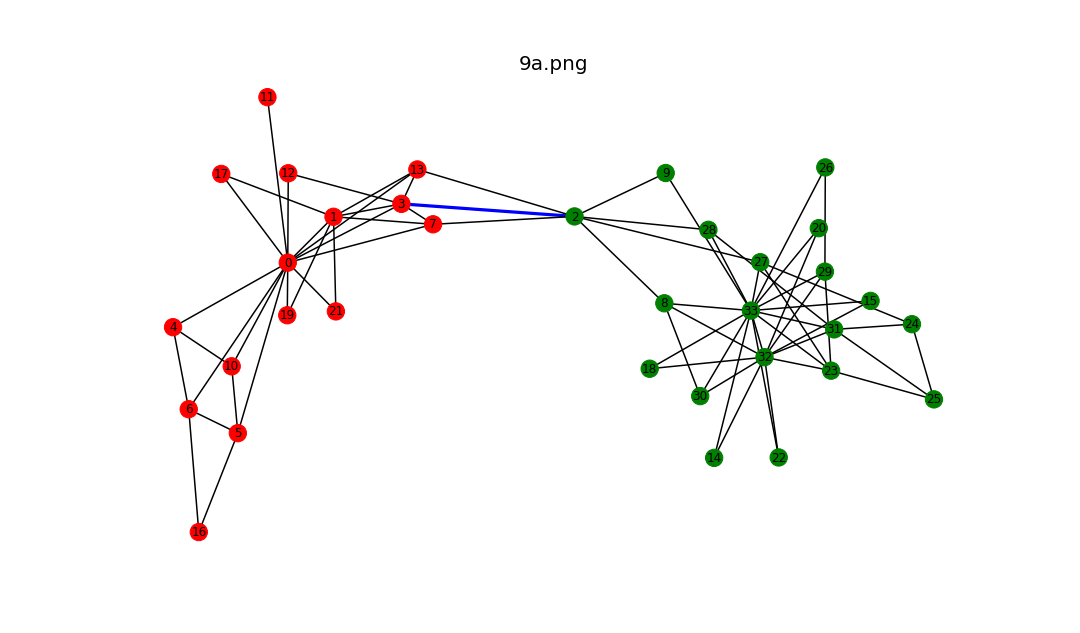
\includegraphics[trim=0 0 0 0, clip, width=\textwidth] {9a.png}
\caption{Iteration 9 Highlighted nodeedge to remove in blue }
\label{fig:q19a}
\end{figure}
\begin{figure}[H]
\centering
% trim and clip are used to crop the image, trim=left bottom right top
% width sets max width, height will be scaled appropriately
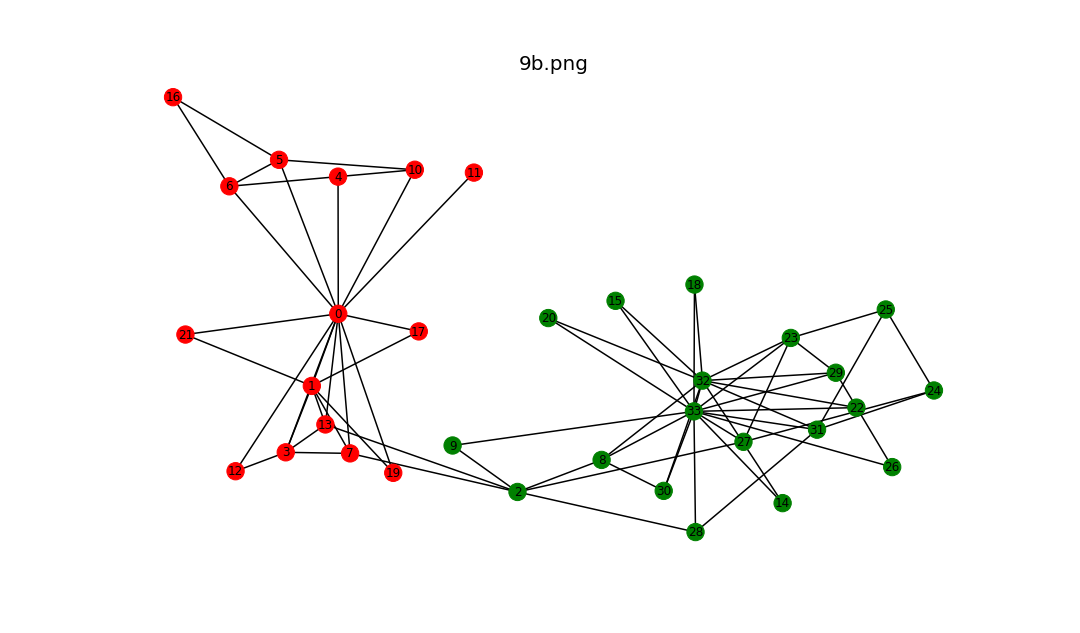
\includegraphics[trim=0 0 0 0, clip, width=\textwidth] {9b.png}
\caption{Iteration 9 confirm nodeedge has been removed }
\label{fig:q19b}
\end{figure}

\begin{figure}[H]
\centering
% trim and clip are used to crop the image, trim=left bottom right top
% width sets max width, height will be scaled appropriately
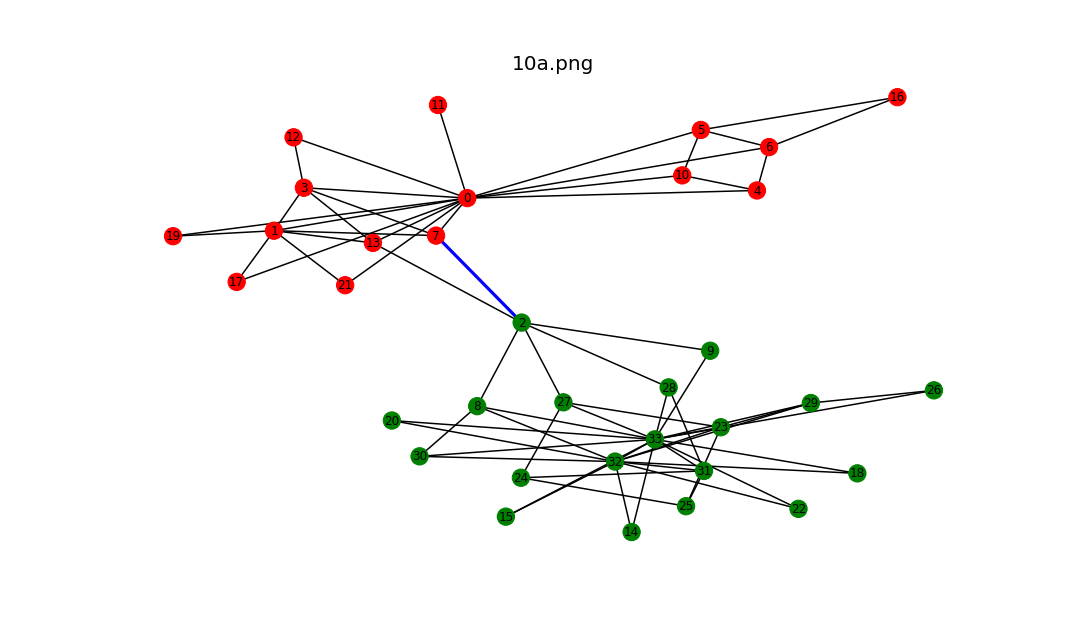
\includegraphics[trim=0 0 0 0, clip, width=\textwidth] {10a.png}
\caption{Iteration 10 Highlighted nodeedge to remove in blue }
\label{fig:q110a}
\end{figure}
\begin{figure}[H]
\centering
% trim and clip are used to crop the image, trim=left bottom right top
% width sets max width, height will be scaled appropriately
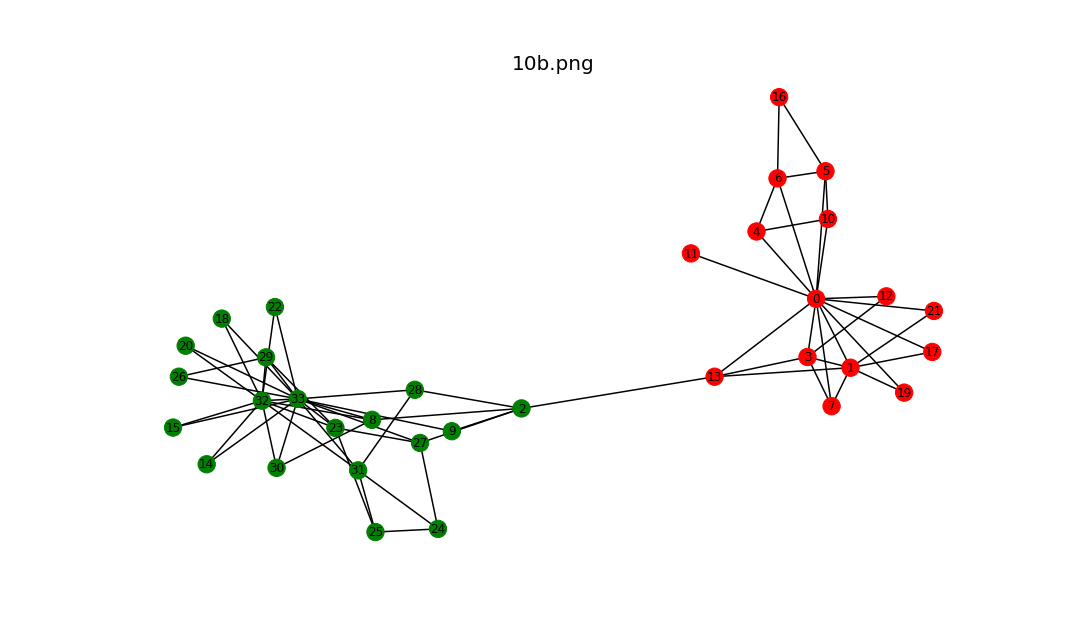
\includegraphics[trim=0 0 0 0, clip, width=\textwidth] {10b.png}
\caption{Iteration 10 confirm nodeedge has been removed }
\label{fig:q110b}
\end{figure}

\begin{figure}[H]
\centering
% trim and clip are used to crop the image, trim=left bottom right top
% width sets max width, height will be scaled appropriately
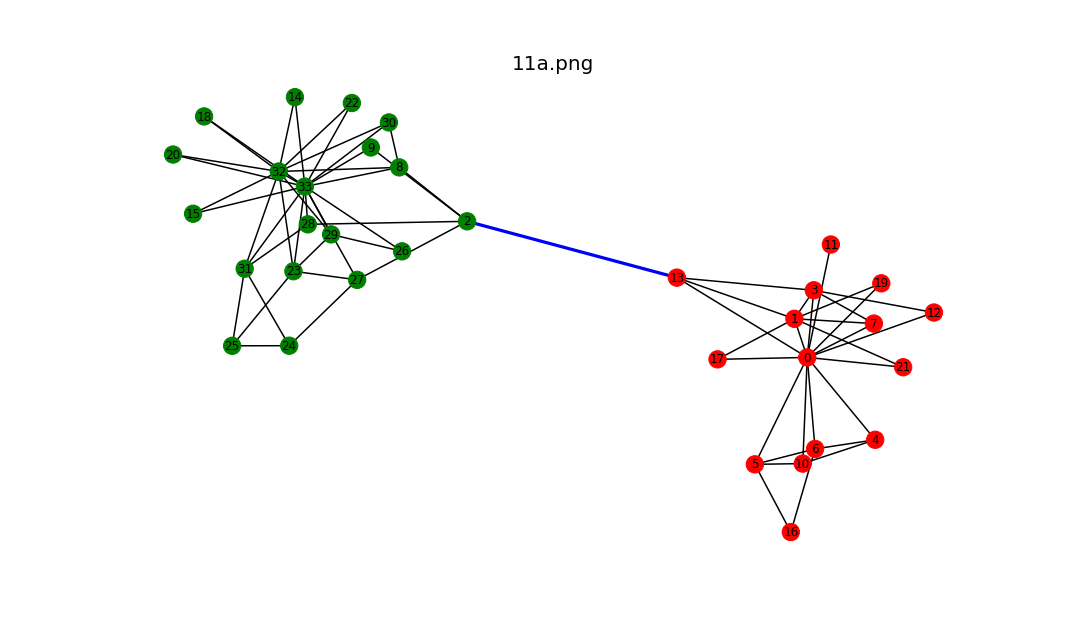
\includegraphics[trim=0 0 0 0, clip, width=\textwidth] {11a.png}
\caption{Iteration 11 Highlighted nodeedge to remove in blue }
\label{fig:q111a}
\end{figure}
\begin{figure}[H]
\centering
% trim and clip are used to crop the image, trim=left bottom right top
% width sets max width, height will be scaled appropriately
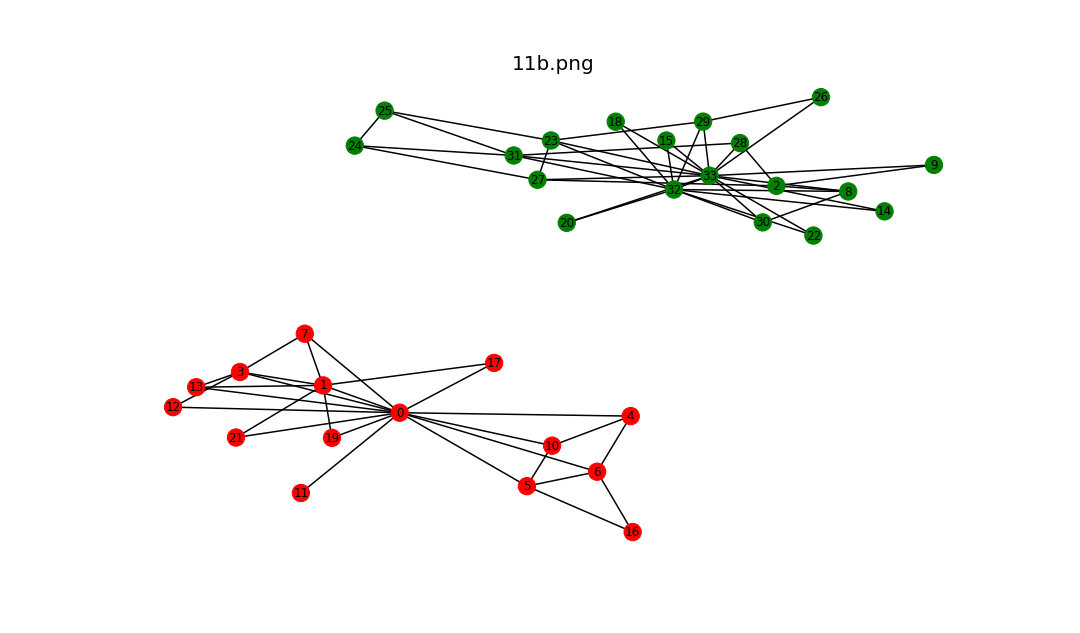
\includegraphics[trim=0 0 0 0, clip, width=\textwidth] {11b.png}
\caption{Iteration 11 confirm nodeedge has been removed }
\label{fig:q111b}
\end{figure}


\subsection*{Discussion}

\emph{It took 11 iteration to complete break the graph into two}


\section*{Q3}
Compare the connected components of the experimental graph (Step 2) with the connected components of the split Karate club graph (Step 1). Are they similar? Did all of the same colored nodes end up in the same group? If not, what is different?
\subsection*{\color{blue}{Answer}}
\begin{figure}[H]
\centering
% trim and clip are used to crop the image, trim=left bottom right top
% width sets max width, height will be scaled appropriately
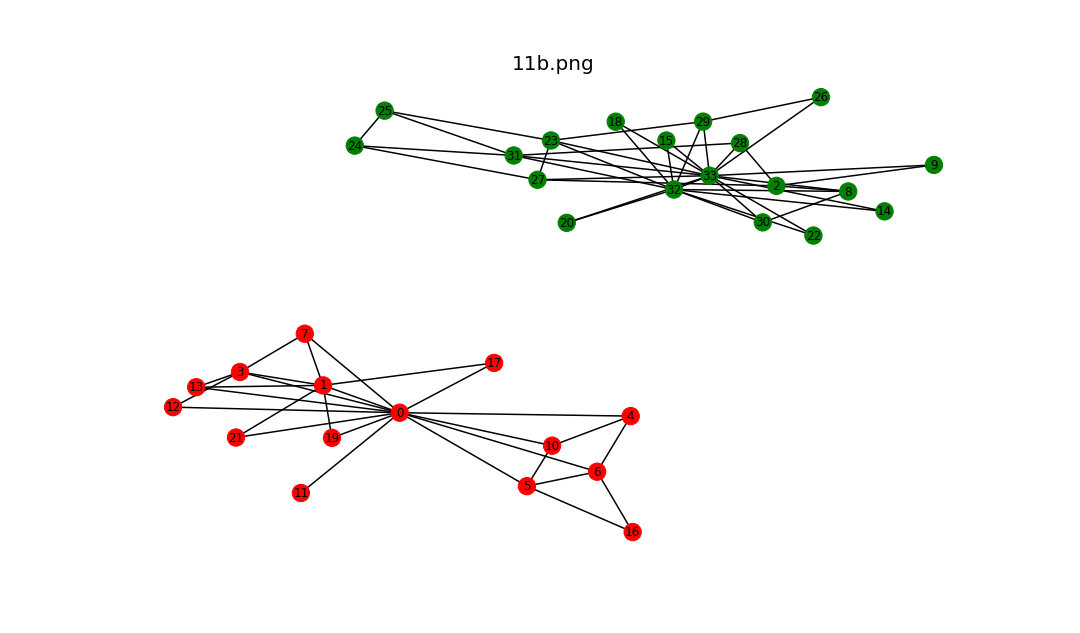
\includegraphics[trim=0 0 0 0, clip, width=\textwidth] {11b.png}
\caption{girvan-newman algorithm final split }
\label{fig:q3a}
\end{figure}

\begin{figure}[H]
\centering
% trim and clip are used to crop the image, trim=left bottom right top
% width sets max width, height will be scaled appropriately
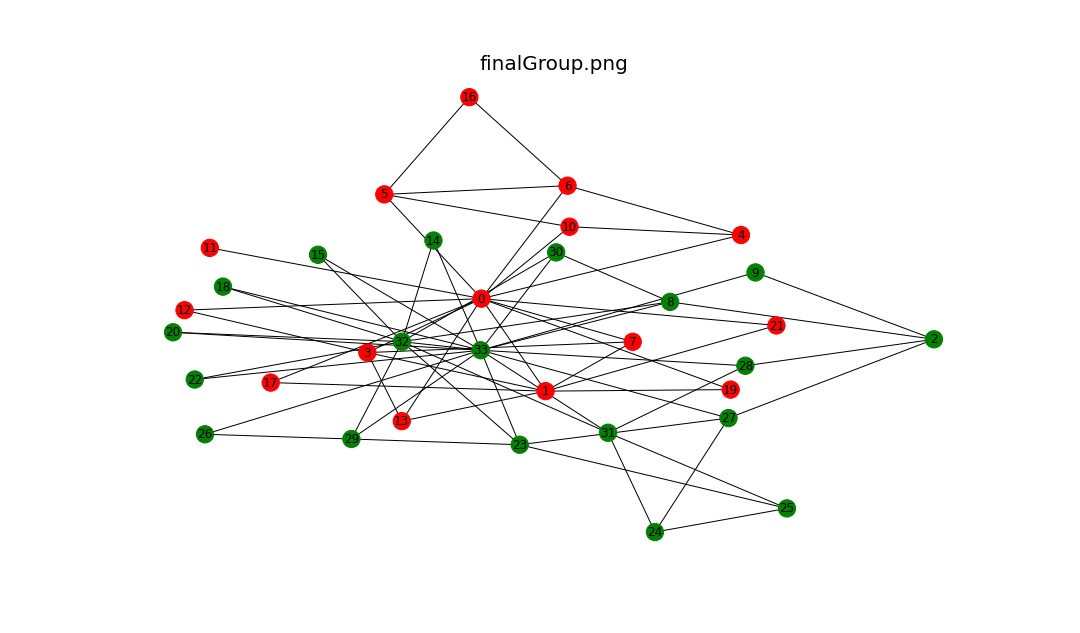
\includegraphics[trim=0 0 0 0, clip, width=\textwidth] {finalGroup.png}
\caption{attached nodesedges with color splitting }
\label{fig:q111b}
\end{figure}
\subsection*{Discussion}

    \begin{itemize}
        \item Are they similar?
        Yes the look very similar to each other 
         \item Did all of the same colored nodes end up in the same group? If not, what is different?
         Yes all the colored node ended up in the same group
         \item The diver of the function
         \lstinputlisting[language=Python,caption=driver for the algorithm (snapshot of graphing.py), label=Q1f:import,firstnumber=136,firstline=136,lastline=153]{graphing.py}
         \item getComponent function in line 146 was used to breakdown the nodes into various node colors of green and red
         \lstinputlisting[language=Python,caption=Get the two NodeView object lists separating them into red and green categories (snapshot of graphing.py), label=Q1f:import,firstnumber=51,firstline=51,lastline=63]{graphing.py}
         \item Used the colorCode funciton to build the node list color based on the result of getComponent
         \item Launched the driver for girvan-new man algorithm on line 151
         \lstinputlisting[language=Python,caption= the driver for newman-algorithm (snapshot of graphing.py), label=Q2:import,firstnumber=151,firstline=151,lastline=151]{graphing.py}
         
        \item In the girvan\_newman function in line 96 to 119 in listing 6
        
        \item Found the maximum edge called it the bestEdge
        \lstinputlisting[language=Python,caption= Best edge finder (snapshot of graphing.py), label=Q2:import,firstnumber=40,firstline=40,lastline=49]{graphing.py}
        \item Built the path for before the removal of edges
        \item Built the edge color list and width of the edge list, to set the color coding and width variable
         \lstinputlisting[language=Python,caption= Setting and reset edges color and width values (snapshot of graphing.py), label=Q2:import,firstnumber=80,firstline=80,lastline=95]{graphing.py}
        \item Made the first Plot using the plot function 
        \item Reset the colors and width to original state
        \item Built the path for after the removal of edges
        \item \lstinputlisting[language=Python,caption= logic in the algorithm (snapshot of graphing.py), label=Q2:import,firstnumber=102,firstline=102,lastline=116]{graphing.py}
        
    \end{itemize}
    
\section*{Extra Credit Q 1}
We know the group split in two different groups. Suppose the disagreements in the group were more nuanced. What would the clubs look like if they split into 3, 4, and 5 groups? A single node can be considered as a "group".
\subsection*{\color{blue}{Answer}}
\begin{figure}[H]
\centering
% trim and clip are used to crop the image, trim=left bottom right top
% width sets max width, height will be scaled appropriately
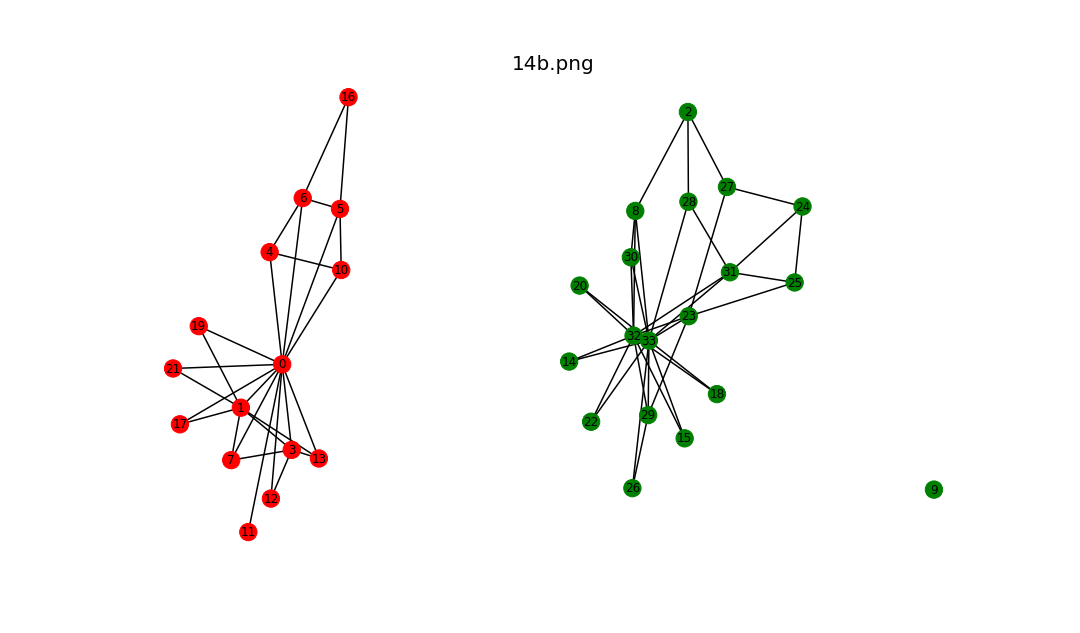
\includegraphics[trim=0 0 0 0, clip, width=\textwidth] {14b.png}
\caption{Group 3}
\label{fig:q3}
\end{figure}
\begin{figure}[H]
\centering
% trim and clip are used to crop the image, trim=left bottom right top
% width sets max width, height will be scaled appropriately
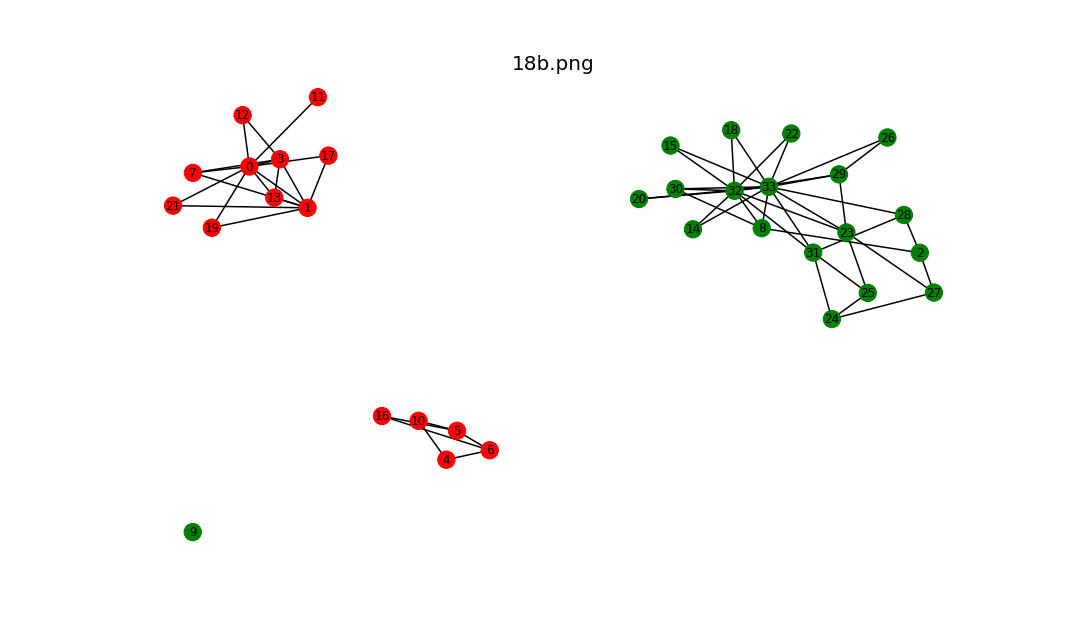
\includegraphics[trim=0 0 0 0, clip, width=\textwidth] {18b.png}
\caption{Group 4 }
\label{fig:q4}
\end{figure}
\begin{figure}[H]
\centering
% trim and clip are used to crop the image, trim=left bottom right top
% width sets max width, height will be scaled appropriately
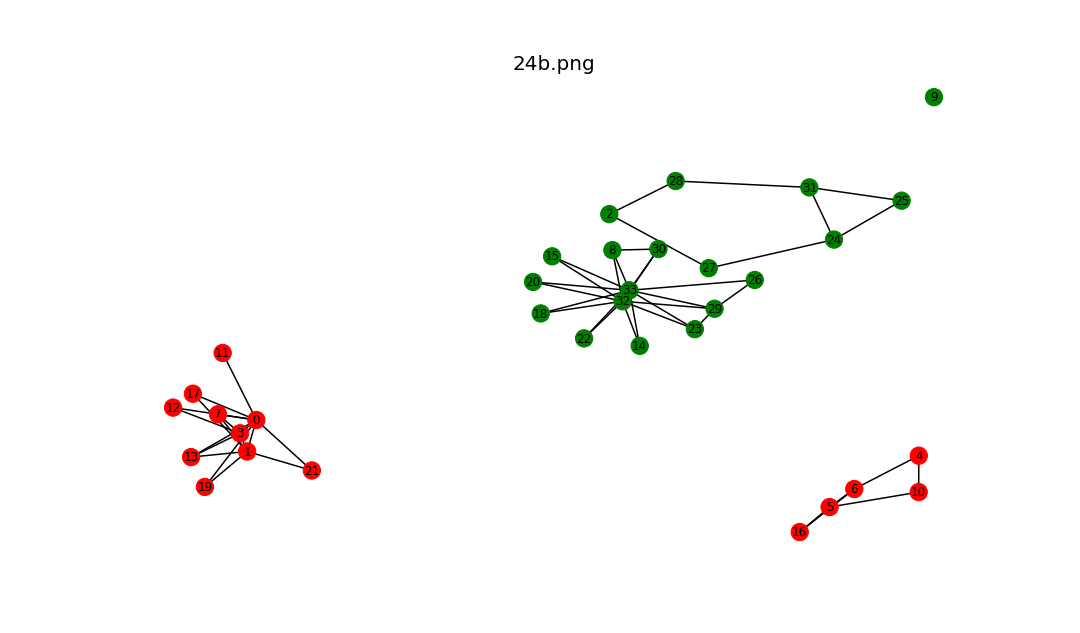
\includegraphics[trim=0 0 0 0, clip, width=\textwidth] {24b.png}
\caption{ Group 5}
\label{fig:q5}
\end{figure}
\subsection*{Discussion}
\emph{Same algorithm of previous question produced these outputs. All output will be included in github}

\section*{References}
\begin{itemize}
    \item {\url{https://stackoverflow.com/questions/9012487/matplotlib-pyplot-savefig-outputs-blank-image}}
     \item {\url{https://gawron.sdsu.edu/python_for_ss/course_core/book_draft/Social_Networks/Networkx.html}}
     \item{\url{https://stackoverflow.com/questions/332289/how-do-you-change-the-size-of-figures-drawn-with-matplotlib}}
     \item{\url{https://networkx.org/documentation/stable/reference/algorithms/generated/networkx.algorithms.community.centrality.girvan_newman.html}}
     \item{\url{https://networkx.org/documentation/stable/tutorial.html}}
     \item{\url{https://networkx.org/documentation/stable/reference/drawing.html#module-networkx.drawing.nx_pylab}}
     
    
     
\end{itemize}

\end{document}

